%\documentclass[gray]{jmlr} % test grayscale version
%\documentclass[tablecaption=bottom]{jmlr}% journal article
\documentclass[pmlr,twocolumn,10pt]{jmlr} % W&CP article

% The following packages will be automatically loaded:
% amsmath, amssymb, natbib, graphicx, url, algorithm2e

%\usepackage{rotating}% for sideways figures and tables
%\usepackage{longtable}% for long tables

% The booktabs package is used by this sample document
% (it provides \toprule, \midrule and \bottomrule).
% Remove the next line if you don't require it.

\usepackage{booktabs}
% The siunitx package is used by this sample document
% to align numbers in a column by their decimal point.
% Remove the next line if you don't require it.
%\usepackage[load-configurations=version-1]{siunitx} % newer version 
\usepackage{siunitx}

% The lineno package is required for denoting line
% numbers for paper review.
\usepackage[switch]{lineno}

% The following command is just for this sample document:
\newcommand{\cs}[1]{\texttt{\char`\\#1}}% remove this in your real article

% The following is to recognise equal contribution for authorship
\newcommand{\equal}[1]{{\hypersetup{linkcolor=black}\thanks{#1}}}

% Define an unnumbered theorem just for this sample document for
% illustrative purposes:
\theorembodyfont{\upshape}
\theoremheaderfont{\scshape}
\theorempostheader{:}
\theoremsep{\newline}
\newtheorem*{note}{Note}

% The optional argument of \title is used in the header
\title[Short Title]{Yolov5 and Yolov8 on the Raspberry PI\titlebreak Comparing execution time of object detection with varying brightness and contrast}

% Anything in the title that should appear in the main title but 
% not in the article's header or the volume's table of
% contents should be placed inside \titletag{}

%\title{Title of the Article\titletag{\thanks{Some footnote}}}


% Use \Name{Author Name} to specify the name.
% If the surname contains spaces, enclose the surname
% in braces, e.g. \Name{John {Smith Jones}} similarly
% if the name has a "von" part, e.g \Name{Jane {de Winter}}.
% If the first letter in the forenames is a diacritic
% enclose the diacritic in braces, e.g. \Name{{\'E}louise Smith}

% \thanks must come after \Name{...} not inside the argument for
% example \Name{John Smith}\nametag{\thanks{A note}} NOT \Name{John
% Smith\thanks{A note}}

% Anything in the name that should appear in the title but not in the 
% article's header or footer or in the volume's
% table of contents should be placed inside \nametag{}

% Two authors with the same address
% \author{%
%  \Name{Author Name1\nametag{\thanks{A note}}} \Email{abc@sample.com}\and
%  \Name{Author Name2} \Email{xyz@sample.com}\\
%  \addr Address
% }

% Three or more authors with the same address:
% \author{%
%  \Name{Author Name1} \Email{an1@sample.com}\\
%  \Name{Author Name2} \Email{an2@sample.com}\\
%  \Name{Author Name3} \Email{an3@sample.com}\\
%  \Name{Author Name4} \Email{an4@sample.com}\\
%  \Name{Author Name5} \Email{an5@sample.com}\\
%  \Name{Author Name6} \Email{an6@sample.com}\\
%  \Name{Author Name7} \Email{an7@sample.com}\\
%  \Name{Author Name8} \Email{an8@sample.com}\\
%  \Name{Author Name9} \Email{an9@sample.com}\\
%  \Name{Author Name10} \Email{an10@sample.com}\\
%  \Name{Author Name11} \Email{an11@sample.com}\\
%  \Name{Author Name12} \Email{an12@sample.com}\\
%  \Name{Author Name13} \Email{an13@sample.com}\\
%  \Name{Author Name14} \Email{an14@sample.com}\\
%  \addr Address
% }

% Authors with different addresses and equal first authors:
\author{%
\Name{Ruben Torres Romero}\equal{These authors contributed equally} \Email{rubent@cpp.edu}\\
\addr Cal Poly Pomona, USA
\AND
% footnotemark[1] is to refer to the \equal footnote
\Name{Ryan Caran Dang}\footnotemark[1] \Email{rrcarendang@cpp.edu}\\
\addr Cal Poly Pomona, USA
\AND
\Name{Ariel Suarez}\footnotemark[1] \Email{suarez@cpp.edu}\\
\addr Cal Poly Pomona, USA
\AND
\Name{Leslie Lin} \Email{lllin.@cpp.edu}\\
\addr Cal Poly Pomona, USA
}

%%%%%%%%%%%%%%%%%%%%%%%%%%%%%%%%%%%%%%%%%%%%%%%%%%%%%%%%%%%%%%%%%%%%%%%%
%%%%%%%%%%%%% Remove the \linenumbers in the final version %%%%%%%%%%%%%
%%%%%%%%%%%%%%%%%%%%%%%%%%%%%%%%%%%%%%%%%%%%%%%%%%%%%%%%%%%%%%%%%%%%%%%%
\linenumbers % Activate line numbering

\begin{document}

\maketitle

\begin{abstract}
YOLO is an object detection and image segmentation model first launched in 2015 by Ali Farhadi at the University of Washington and it gained popularity due to its high accuracy and performance. Image segmentation is a computer vision task that divides images into multiple regions based on characteristics such as color and the goal is to simplify the representation of the image into something meaningful so it can be easily analyzed. The fundamental idea behind YOLO is to view object detection as a regression problem. YOLO divides the image into a grid and directly predicts bounding boxes and class probabilities for each grid cell. There are currently eight YOLO versions. YOLOv5 launched in 2020 improved the model's performance and added features such as hyper parameter optimization, integrated experiment tracking, and automatic export. YOLOv8 is the latest version and supports many AI tasks and has advanced backbone and neck architectures. 
\end{abstract}

\paragraph*{Data and Code Availablity}
Data is from the public data set in Roboflow. 
\url{https://universe.roboflow.com/tank-kbbhk/tank-detect}. 
Code used to train on google colab and run on the raspberry pi is contained in following github
\url{https://github.com/chihuahuadog/ece4300project.git}. 

\section{Introduction}
\label{sec:intro}
The goal is to compare the performance of YOLOv5 and YOLOv8 on a specific tank data set. Google Colab is used to train YOLOv8 and YOLOv5 on a particular data set acquired from Roboflow, as the Raspberry PI lacks sufficient computing resources to develop a robust model. Using the two generated models, the tank is detected in a set containing six images, and the execution time is measured using the time module in Python for each image.

To assess the robustness of the models, variations in image characteristics are introduced. Firstly, image brightness is adjusted by factors of 1.2 and 1.5, subjecting the models to these brightness-adjusted images to evaluate their adaptability to varying lighting conditions. In a parallel experiment, the impact of contrast adjustments on model performance is investigated. To maintain experimental rigor, these contrast adjustments are applied exclusively to the original images, excluding those subjected to brightness modifications. Similar to the brightness experiment, adjustments are made at factors of 1.2 and 1.5, and the models are tasked with identifying tanks in these contrast-adjusted images.
\begin{note}
YOLOv8 and YOLOv5 may perform differently depending on dataset so our results may not be applicable in all cases.
\end{note}

\section{Comparing YOLOv8 and YOLOv5 on original images}

Mentioned earlier, a set of six tank images is processed through YOLOv8 and YOLOv5, and the execution time is measured. For YOLOv8, the confidence scores (probabilities) for the images are 0.90, 0.92, 0.93, 0.87, 0.89, and 0.89. The execution times for the images are 15.09, 9.64, 9.14, 8.67, 7.87, and 8.23, with an average time of 9.77 seconds. For YOLOv5, the confidence scores for the images are 0.96, 0.91, 0.75, 0.91, 0.95, and 0.94. The execution times for the images are 32.22, 24.00, 22.38, 23.62, 22.67, and 22.01, with an average of 24.32 seconds. Generally, the confidence score is higher for YOLOv5, but the execution time is approximately twice as long as YOLOv8.

\section{Adjusting Brightness}
The brightness of the images is adjusted by running them through a Python program that utilizes the ImageEnhance function from the PILLOW module in Python. The adjustment factors used are 1.2 and 1.5.

\subsection{Adjusting brightness in YOLOv8}
\label{sec:figures}

For the brightness adjustment of 1.2, the execution times for the images are 9.58s, 10.32s, 8.63s, 8.44s, 8.07s, and 7.97s, with an average of 8.83s, which is less time than it took for YOLOv8 to run on the original images. However, the confidence scores are much lower with the following scores: 0.92, 0.86, 0.93, 0.89, 0.88, and 0.90.

For the brightness adjustment of 1.5, the execution times for the images are 9.31s, 9.53s, 8.98s, 8.75s, 8.67s, and 8.21s, with an average of 8.91s, which is less time than it took for YOLOv8 to run on the original images but longer than the brightness adjustment of 1.2. However, the confidence scores are much lower with the following scores: 0.91, 0.87, 0.93, 0.85, 0.85, and 0.87.

\begin{figure}[htbp]
 % Caption and label go in the first argument and the figure contents
 % go in the second argument
\floatconts
  {fig:nodes}
  {\caption{Results for brightness adjust of 1.2}}
  {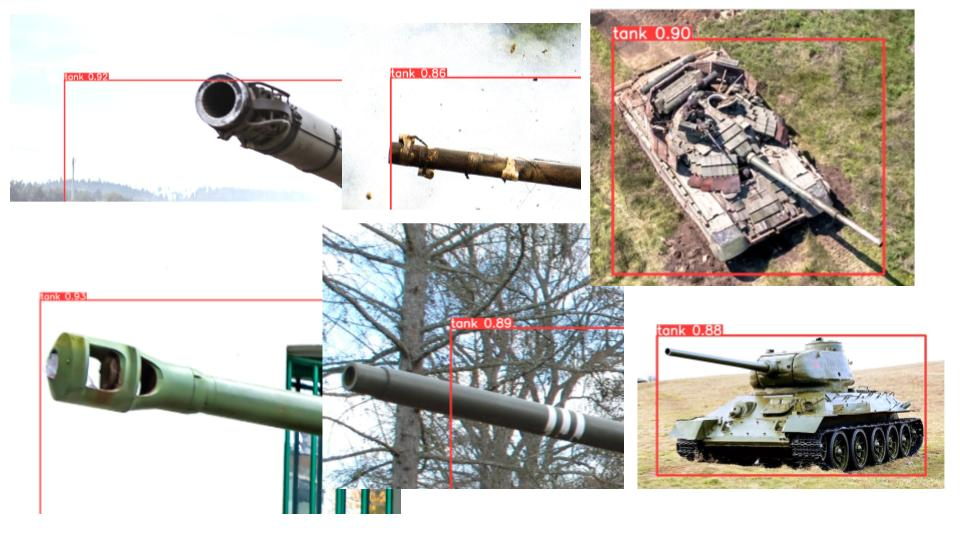
\includegraphics[width=1\linewidth]{images/Yolo8Bright12.jpg}}
\end{figure}

\begin{figure}[htbp]
\floatconts
  {fig:nodes}
  {\caption{Results for brightness adjust of 1.5}}
  {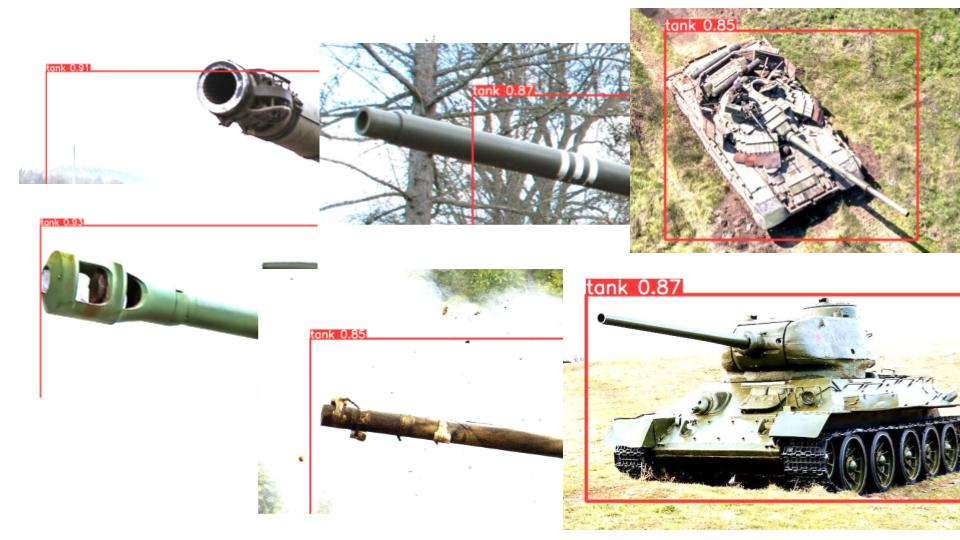
\includegraphics[width=1\linewidth]{images/Yolo8Bright15.jpg}}
\end{figure}

\subsection{Adjusting brightness in YOLOv5}
\label{sec:figures}

For the brightness adjustment of 1.2, the execution times for the images are 23.13s, 23.62s, 22.37s, 21.34s, 23.50s, and 21.66s, with an average of 22.60s, which is less time than it took for YOLOv5 to run on the original images. The confidence scores are also higher with the following scores: 0.93, 0.77, 0.74, 0.95, 0.96, and 0.91.

For the brightness adjustment of 1.5, the execution times for the images are 23.10s, 22.50s, 22.75s, 22.76s, 22.90s, and 22.74s, with an average of 22.79s, which is less time than it took for YOLOv5 to run on the original images but slightly longer than the brightness adjustment of 1.2. The confidence scores are much lower than the brightness adjustment of 1.2 but higher than the original images, with the following scores: 0.93, 0.77, 0.74, 0.95, 0.96, and 0.91.

\begin{figure}[htbp]
 % Caption and label go in the first argument and the figure contents
 % go in the second argument
\floatconts
  {fig:nodes}
  {\caption{Results for brightness adjust of 1.2}}
  {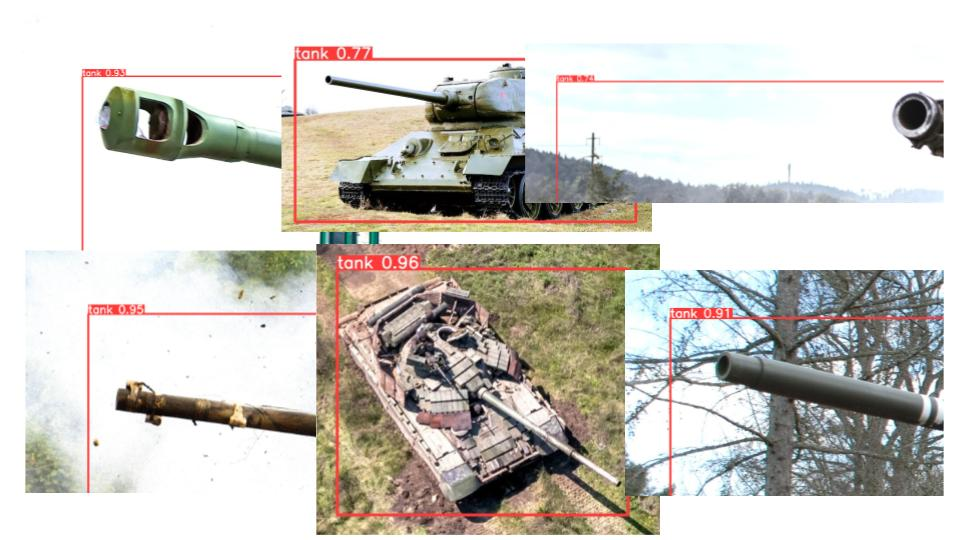
\includegraphics[width=1\linewidth]{images/Yolo5Bright12.jpg}}
\end{figure}

\begin{figure}[htbp]
\floatconts
  {fig:nodes}
  {\caption{Results for brightness adjust of 1.5}}
  {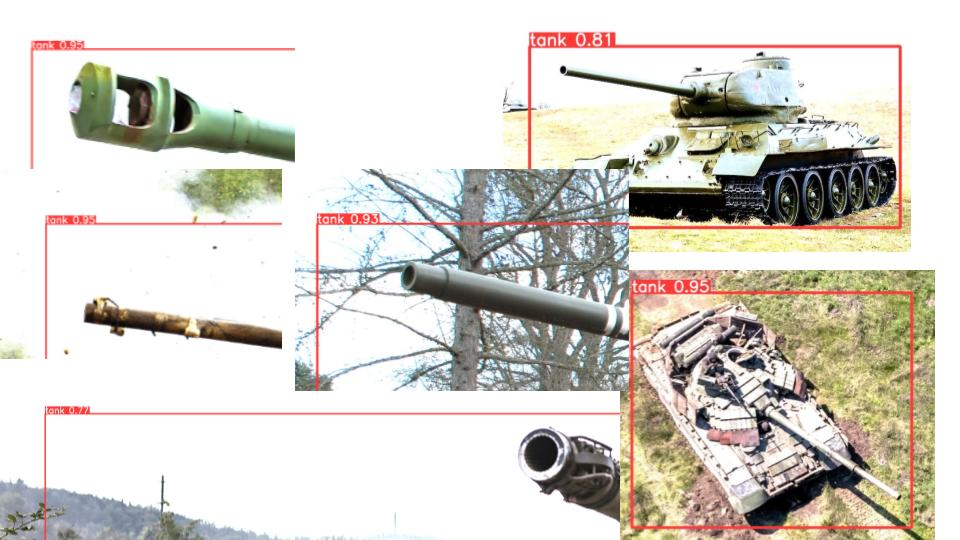
\includegraphics[width=1\linewidth]{images/Yolo5Bright15.jpg}}
\end{figure}

\section{Adjusting Contrast}
The contrast of the images is adjusted by running them through a Python program that utilizes the ImageEnhance function from the PILLOW module in Python. The adjustment factors used are 1.2 and 1.5.

\subsection{Adjusting Contrast in YOLOv8}
\label{sec:figures}

For the contrast adjustment of 1.2, the execution times for the images are 8.72s, 9.73s, 9.98s, 8.93s, 8.84s, and 8.22s, with an average of 9.09s, which is slightly less time than it took for YOLOv8 to run on the original images. However, the confidence scores are lower with the following scores: 0.91, 0.92, 0.86, 0.89, 0.89, and 0.86.

For the contrast adjustment of 1.5, the execution times for the images are 9.73s, 9.98s, 8.93s, 8.94s, 8.22s, and 8.72s, with an average of 9.09s, which is less time than it took for YOLOv8 to run on the original images and about the same time as the contrast adjustment of 1.2. However, the confidence scores are much lower with the following scores: 0.91, 0.86, 0.84, 0.76, 0.85, and 0.78.

\begin{figure}[htbp]
 % Caption and label go in the first argument and the figure contents
 % go in the second argument
\floatconts
  {fig:nodes}
  {\caption{Results for contrast adjust of 1.2}}
  {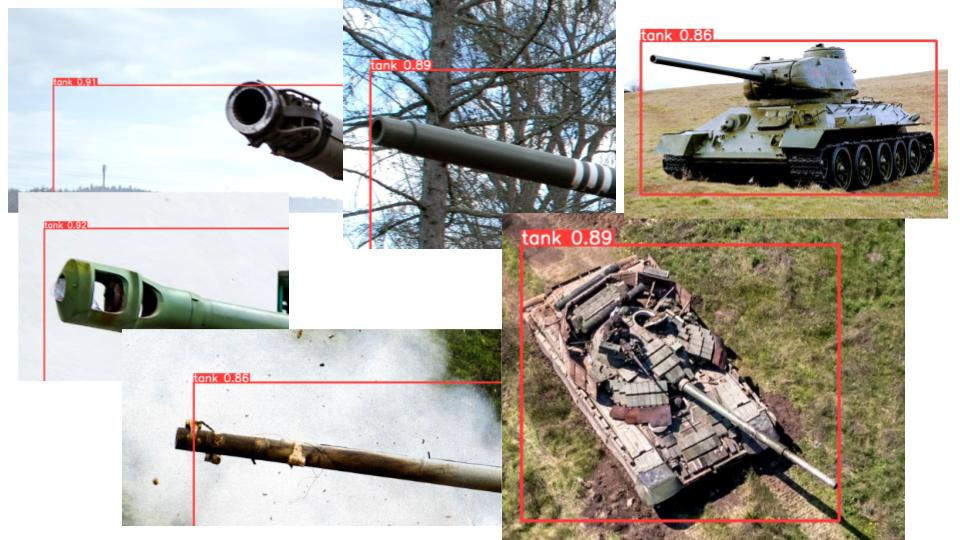
\includegraphics[width=1\linewidth]{images/Yolo8Con12.jpg}}
\end{figure}

\begin{figure}[htbp]
\floatconts
  {fig:nodes}
  {\caption{Results for contrast adjust of 1.5}}
  {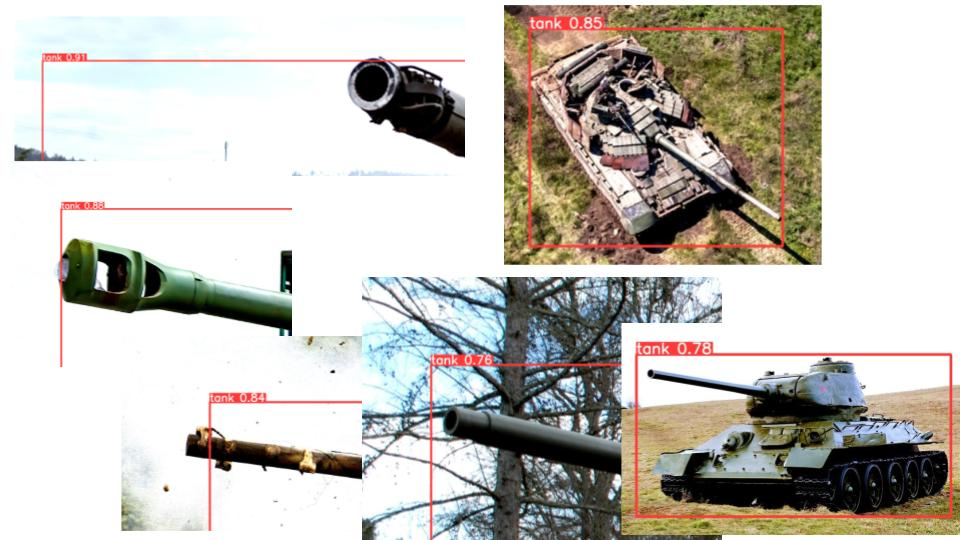
\includegraphics[width=1\linewidth]{images/Yolo8Con15.jpg}}
\end{figure}

\subsection{Adjusting Contrast in YOLOv5}
\label{sec:figures}
For the contrast adjustment of 1.2, the execution times for the images are 22.53s, 22.64s, 23.34s, 22.26s, 22.46s, and 22.96s, with an average of 22.70s, which is less time than it took for YOLOv5 to run on the original images (24.32s). The confidence scores are also generally higher with the following scores: 0.95, 0.95, 0.95, 0.91, 0.72, and 0.92.

For the contrast adjustment of 1.5, the execution times for the images are 21.94s, 23.86s, 23.35s, 21.61s, 22.38s, and 22.07s, with an average of 22.40s, which is less time than it took for YOLOv5 to run on the original images and the contrast adjustment of 1.2. However, the confidence scores are much lower than the original images and the contrast adjustment of 1.2 images, with the following scores: 0.92, 0.87, 0.95, 0.65, 0.79, and 0.95.

\begin{figure}[htbp]
 % Caption and label go in the first argument and the figure contents
 % go in the second argument
\floatconts
  {fig:nodes}
  {\caption{Results for contrast adjust of 1.2}}
  {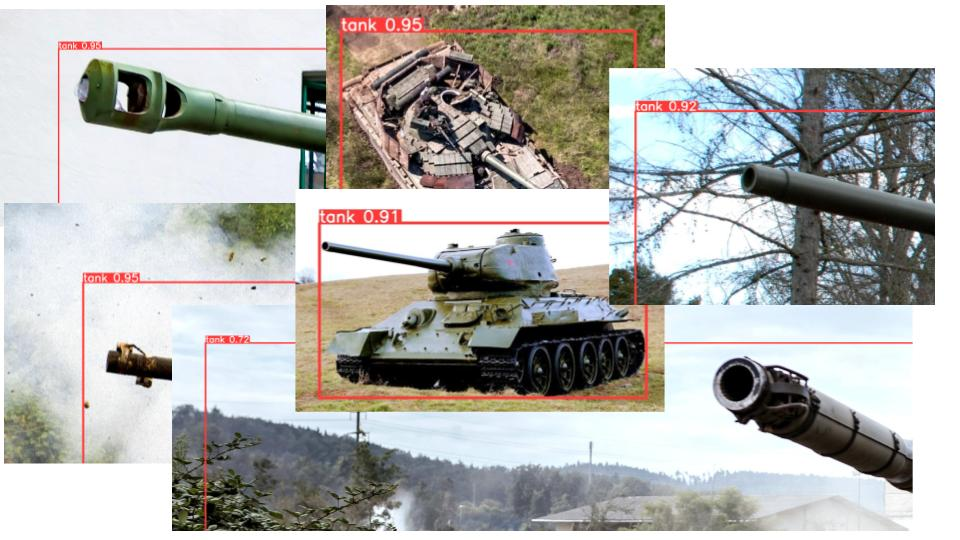
\includegraphics[width=1\linewidth]{images/Yolo5Con12.jpg}}
\end{figure}

\begin{figure}[htbp]
\floatconts
  {fig:nodes}
  {\caption{Results for contrast adjust of 1.5}}
  {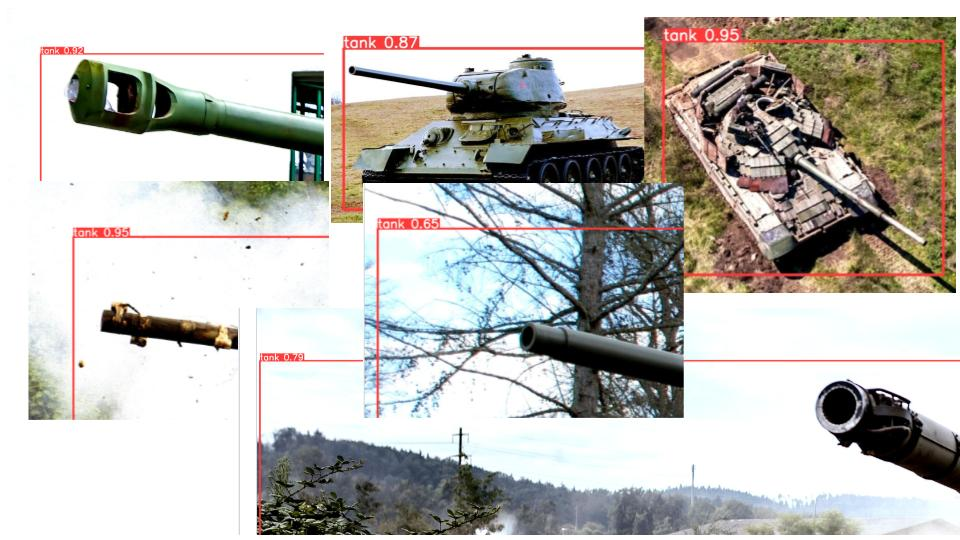
\includegraphics[width=1\linewidth]{images/Yolo5Con15.jpg}}
\end{figure}

\section{Conclusion}
In this study, a comparative analysis is conducted on YOLOv5 and YOLOv8 using a specific tank dataset to assess their performance on the Raspberry Pi. Due to computational limitations on the Raspberry Pi, the models are trained on Google Colab. The analysis includes original images and variations introduced by adjusting brightness and contrast.

The examination of original images reveals that YOLOv8 exhibits faster execution times compared to YOLOv5, while YOLOv5 generally achieves higher confidence scores. The trade-off between speed and accuracy is crucial for real-time object detection applications, and the choice between the two models may depend on specific project requirements.

Additionally, the study explores the adaptability of the models to varying image characteristics introduced by adjusting brightness and contrast. This testing of robustness shows that both YOLOv5 and YOLOv8 demonstrate a degree of resilience to these variations, with varying impacts on execution times and confidence scores.

It is essential to recognize that the results are specific to the chosen tank dataset and may not be directly applicable to other scenarios. The performance of YOLOv5 and YOLOv8 can be influenced by the dataset's nature, and users are encouraged to conduct model evaluations based on their specific use cases.

In conclusion, this research provides insights into the comparative performance of YOLOv5 and YOLOv8 on the Raspberry Pi, laying a foundation for further exploration and optimization in the realm of real-time object detection.
\section{Citations and Bibliography}
1)\url{https://github.com/ultralytics/ultralytics}
2)\url{https://github.com/ultralytics/yolov5}

3)\url{https://blog.roboflow.com/yolov5-improvements-and-evaluation/}
4)\url{https://yolov8.com/}
\end{document}
